\paragraph{Цель работы:} Знакомство с CNC-симулятором G-code. Изучение программы формирования конуса.

\subsection*{Выполнение}

\begin{enumerate}
    \item Знакомство с интерфейсом симулятора
    \item Загрузка программы формирования конуса, изучение программы (рисунок \ref{fig:default}).
    \item Изменение начального и конечного радиусов конуса (рисунок \ref{fig:changed}).
\end{enumerate}

Для формирования конуса используется инструкция перемещения резца из точки с координатами (14, 1) в точку (20, -25). В последующем мы меняем координаты этих точек на (10, 1) и (14, -25) соответственно.

\begin{verbatim}
    N0080 G00 X10.000 Z1.000
    N0090 G01 X14.000 Z-25.000
\end{verbatim}

Скриншоты выполнения лабораторной работы прилагаются в приложении А.

\subsection*{Выводы}

В лабораторной работе мы изучили симулятор CNC G-кода и провели симуляцию формирования конуса стандартной операцией перемещения резца.

\clearpage

\subsection*{Приложение А}

\begin{figure}[ht]
\centering
	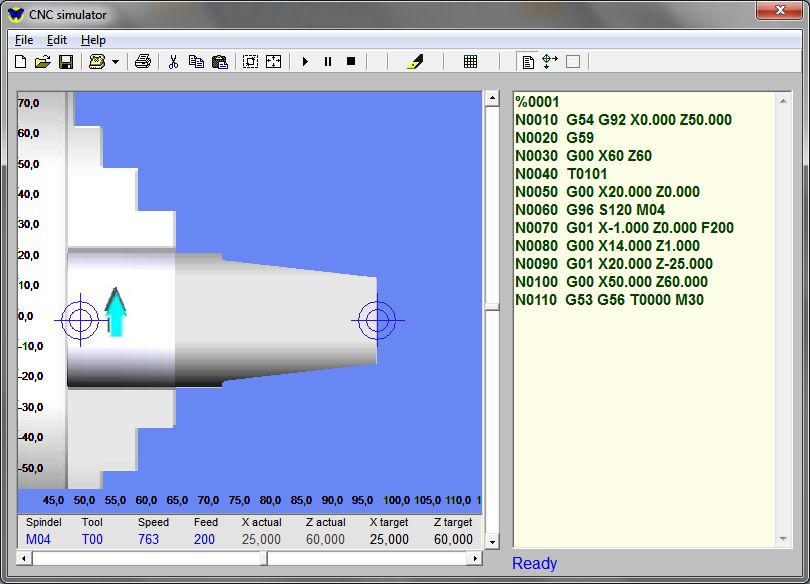
\includegraphics[scale=0.54]{1.png}
    \caption{Формирование стандартного конуса\label{fig:default}}
\end{figure}

\begin{figure}[ht]
\centering
    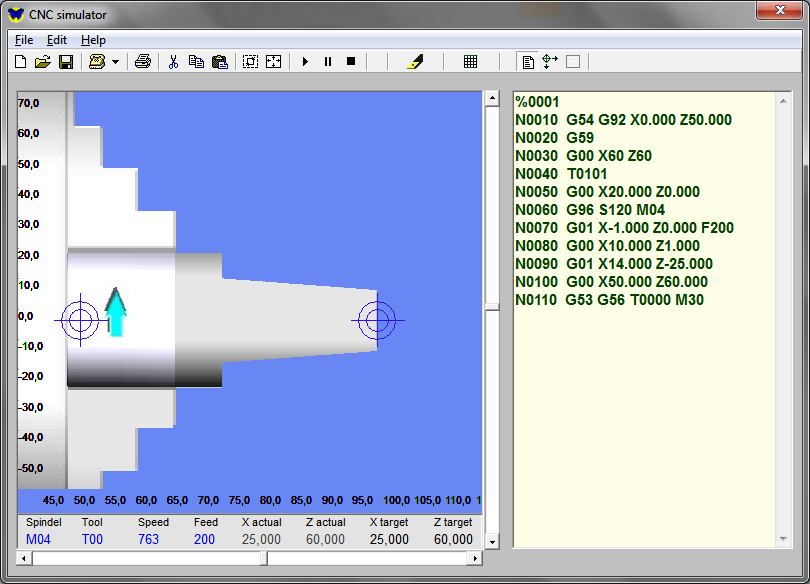
\includegraphics[scale=0.54]{2.png}
    \caption{Формирование измененного конуса\label{fig:changed}}
\end{figure}

\clearpage
